\documentclass[11pt]{article}
\usepackage{graphicx}
\usepackage[legalpaper,landscape, margin=0.4in]{geometry}
\usepackage{multicol}
\usepackage{titlesec}
\usepackage[T1]{fontenc}
\usepackage{upquote}
\titlespacing*{\subsection}
{0pt}{1ex plus 1ex minus .3ex}{0ex}
\titlespacing*{\subsubsection}
{0pt}{1ex plus 1ex minus .3ex}{0ex}
\titleformat{\subsection}
  {\normalfont\fontsize{9}{15}\bfseries}{\thesection}{1em}{}
  \titleformat{\subsubsection}
  {\normalfont\fontsize{8}{15}\bfseries}{\thesection}{1em}{}
\begin{document}
\pagenumbering{None}
\setlength{\columnsep}{1cm}
\begin{multicols*}{3}
\subsection*{Some terms}
Machine translation - predicting which word is used is more frequent \\
 Improvement in perplexity often correlates with improvement in speech recognition performance
\subsection*{Edit distance}
Do row by row
if letter is different, add substitution cost\\
min edit distance at any cell is the cost + 1 from the left cell \\
if letter is same take no cost from i-1, j-1 (diagonal)
\\\\
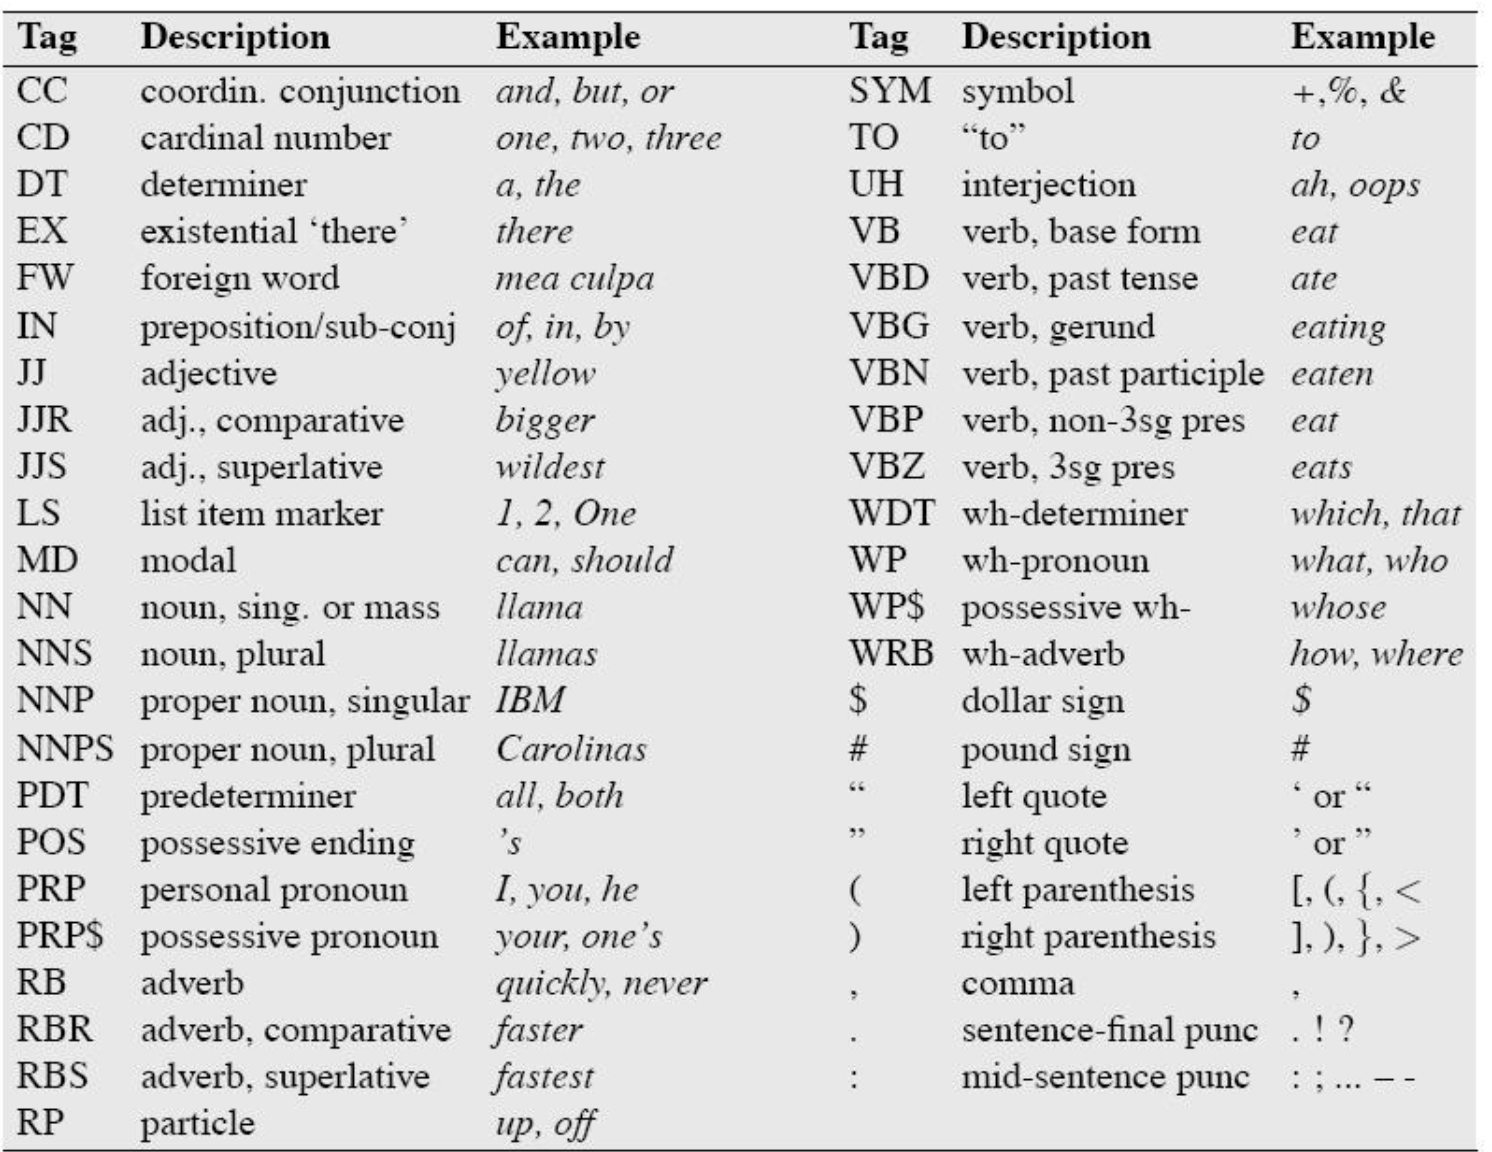
\includegraphics[height=7cm]{images/w.png}
\\
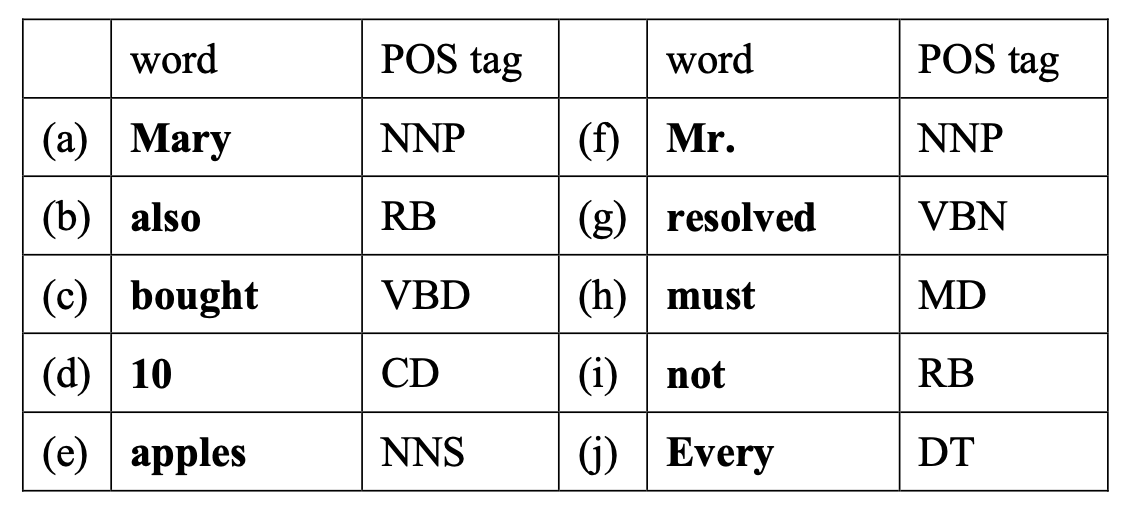
\includegraphics[height=3cm]{images/w1.png}
\subsection*{Personal pronoun}
PRP - He
\subsection*{Auxiliary}
AUX - Does
\subsection*{Determiners (DT)}
the, a, some, that, this\\
E.g. Does that\\\\
particles (RP) can appear after object\\
prepositions (IN) can appear only after verb \\
E.g. of, off, on\\
I thought that/IN
\subsection*{adjectives (JJ)} 
E.g. other, grand, already married/JJ
\subsection*{Verbs}
VBD - commented\\
VBP - do, have\\
VBZ - is\\
There/EX are 70 children there/RB
\subsection*{Modal}\\
MD - could\\
\subsection*{Personal Pronouns}
PRP - you\\
PRP\$ - your
\subsection*{Binary classification}
sign(x) = 1 for x $\geq$ 0, -1 for x $<$ 0
Feature extraction so that there is a good mapping of x
\subsection*{Softmax}
[2 -1 5]\\
\(\frac{e^{2}}{e^{2} + e^{-1} + e^{5}}\) into another vector of 3 numbers where it sum to 1
\\
\subsection*{Loss functions}
$L_{cross-entropy} (\hat{y}, y) = - \sum\limits_{i} y log (\hat{y})$\\
\\
or $- log(\hat{y}) for hard classification$\\
$\hat{y}$ is 1 then it can minimize the loss function\\
$\hat{y}$ requires softmax for transformation\\
\subsection*{Ranking loss}\\
$L_{ranking} (x, x') = max(0, 1 - (f(x) - f(x')))$
\subsection*{Gradient descent}
$w_{i} \leftarrow w_{i} - \alpha \frac{\partial_{L}}{\partial_{w_{i}}}$ for $\alpha >$ 0\\
Successive iterative approximation, can't plug in a value like $w_{1, 1}$\\
if L(w) is convex (single min point), then it will converge to global minimum
\subsection*{Expected number of bits}
\sum bits * P(bits) = $1 \times \frac{1}{2} + 2 \times \frac{1}{4} + 3 \times \frac{1}{8}$ ... = 2
Entropy is the number of bits needed to encode
\subsection*{Per word cross entropy} 
Entropy rate = $\frac{1}{n} H(w_{1}) = -\frac{1}{n} (\sum p(W) log(p(W))$
\subsection*{Smoothing}
$P(w|c_{i}) = \frac{\# times\ w\ occur\ in\ texts\ of\ class\ c_{i}}{\sum \# times w\ occurs\ in\ texts\ of\ class\ c_{i}}$
\\
$P(w|c_{i}) = \frac{\# times\ w\ occur\ in\ texts\ of\ class\ c_{i}\ + 1}{\sum \# times\ w\ occurs\ in\ texts\ of\ class c_{i} + V}$\\
$C^{*}(w_{0} w) = \{C(w_{0} w) + 1\} \times \frac{C(w_0)}{C(w_0) + V} $
\\
\subsubsection*{Witten Bell}
\\
If C^{*}($w_{x}w_{i}$) $>$ 0, $C(w_{x})$ $\times \frac{C(w_{x}w_{i})}{C(w_{x}) + T(w_{x})}$
\\
If C^{*}($w_{x}w_{i}$) $=$ 0, $\frac{ c(w_{x})T(w_{x})}{Z(w_{x}) (c(w_{x}) + T(w_{x}))} $
\subsection*{Stochastic POS tagging}
\)\)
 $P(T,W) = P(<s> , t_{1}, w_{1}, t_{2}, w_{2}...<s>)$\\
= $P(<s>) \cdot P(t_{1} | <s>) \cdot P(w_{1} | <s>, t_{1}) $
\\
$P(T|W) = \frac{P(T, W)}{P(W)} = P(T, W)$
\subsection*{Markov assumption}
$w_{k}$ only depends on the previous n - 1 words\\
$P(w_{k} | w_{1}, .., w_{k-1})$ \approx $P(w_{k}| w_{k-1})$
\subsection*{Vertibi}
v(tag, word) = P(w_{i} | t_{i}) \times P(t_{i} | t_{i-1}) \times P(t_{i-1}) \\
\\
Trigram P(t_{i} |  t_{i-1} t_{i-2}) = P(t_{i} |  t_{i-1} t_{i-2}) + P(t_{i} |  t_{i-1}) + P(t_{i})
\subsection*{Forward computation}
1. Look at the number of input nodes\\
2. Compute the s node which is the value before there is actually $h_{1}$(non-linear activation function)\\\\
$s_{i} = w_{x}i_{i} + w_{x+1}i_{i+1} ... + w_{k}i_{k} + ... b_{i}$\\
For the hidden layers $i_{i}$ will be $h_{i}$\\\\
$h_{i} = \frac{1}{1 + e^{-s_{i}}}$\\
Final value $h_{i}$ will be $o_{i}$
\\\\
$L = \frac{1}{2} \big[ (o_{1} - t_{1})^2 +  (o_{2} - t_{2})^2 \big]$
\subsection*{Backward computation}
\textbf{Base case}\\
1. Take the s values previously computed \\
2. Calculate $\frac{\partial_{L}}{\partial_{w_{m}}} =  \frac{\partial_{L}}{\partial_{s_{1}}}\frac{\partial_{s_{1}}}{\partial_{w_{m}}}$\\
	E.g. $\frac{\partial_{L}}{\partial_{w_{6}}}$\\
	\\$\frac{\partial_{L}}{\partial_{s_{3}}}= (o_{1} - t_{1}) \times o_{1}(1 - o_{1})$\\
$\frac{\partial_{s_{3}}}{\partial_{w_{6}}} = h_{2}$\\\\
\textbf{Recursive case}\\
E.g. $\frac{\partial_{L}}{\partial_{w_{2}}}$\\
\\$\frac{\partial_{L}}{\partial_{w_{2}}}= \frac{\partial_{L}}{\partial_{s_{1}}} \times i_{2}$\\
$\frac{\partial_{L}}{\partial_{s_{1}}} = \big[\frac{\partial_{L}}{\partial_{s_{3}}} \times w_{5} + \frac{\partial_{L}}{\partial_{s_{4}}} \times w_{7} \big] \times h_{1}(1 - h_{1})$\\
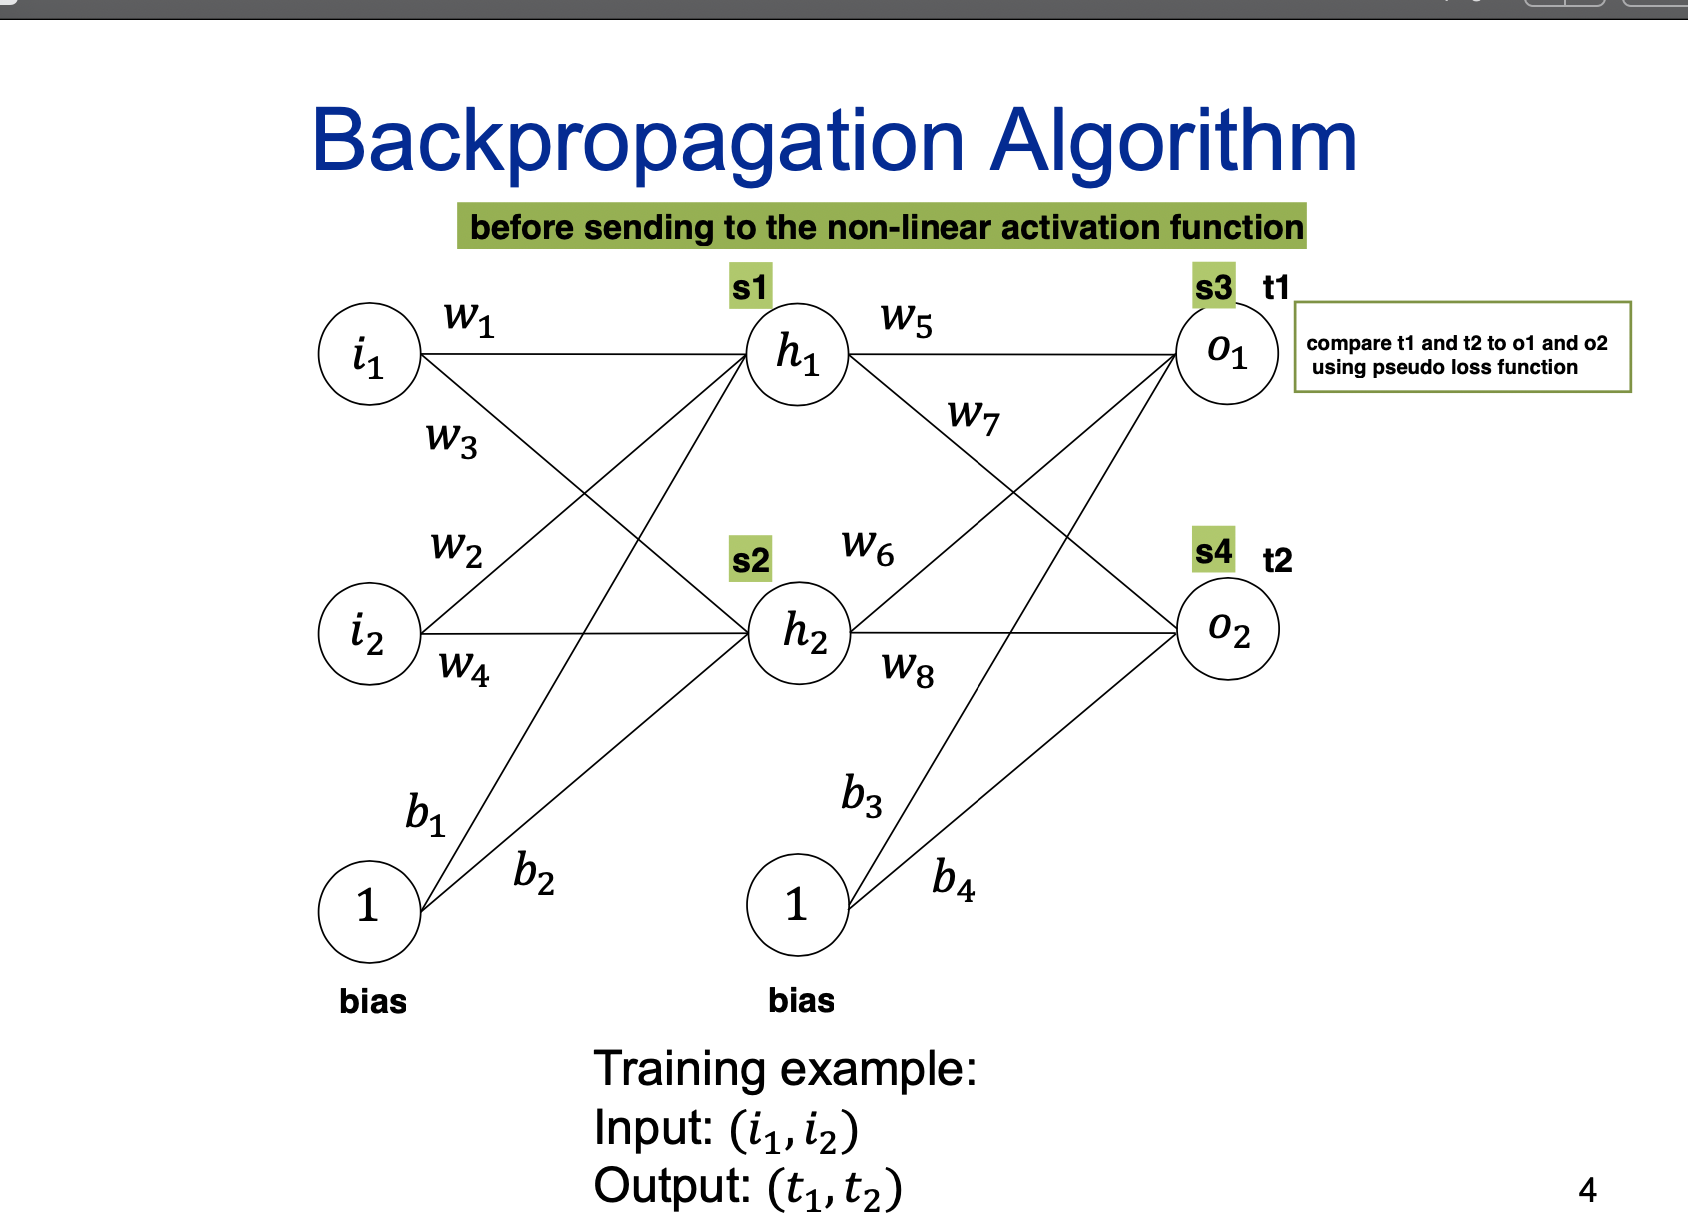
\includegraphics[height=7cm]{images/b}\\
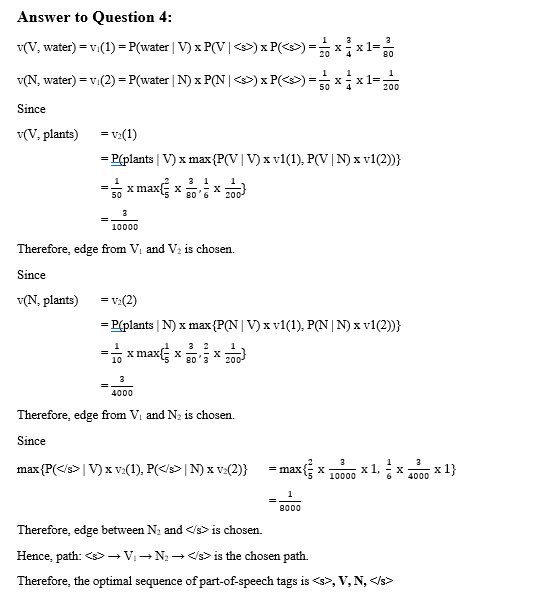
\includegraphics[height=10cm]{images/ver}\\
\subsection*{CFG}
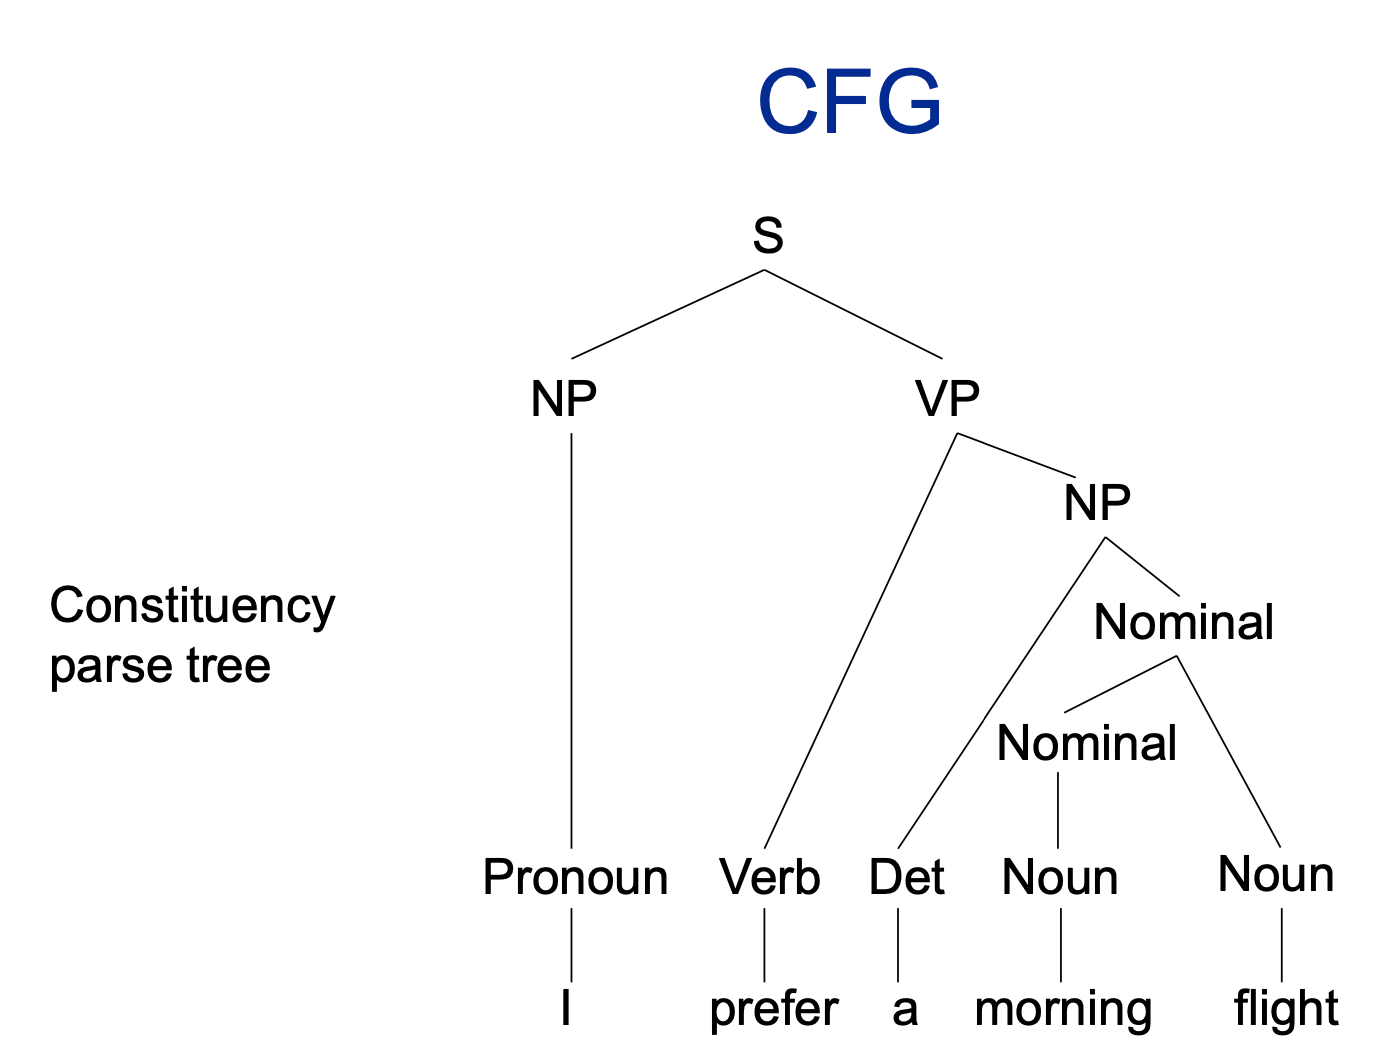
\includegraphics[height=5.5cm]{images/w4}\\

\includegraphics[height=1.8cm]{images/w5}\\
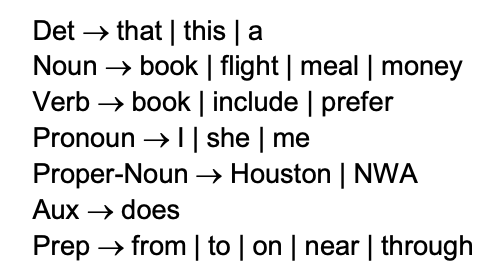
\includegraphics[height=2cm]{images/w6}
\subsection*{CKY - Bottom up}
1. Define base case where non-terminal expands into a word\\
2. For a computed cell, try every combination for e.g. [1, 5] is there a rule at cell [1, 5] that expands to [1, 2] and [2, 5], [1, 3] and [3, 5]\\
\textquotesingle a flight through\textquotesingle\ is not a constituent then there would be no symbol assigned
\subsection*{Earley algorithm}
1. Write down in chart[0] where RHS is non-terminal symbol\\
!Note! Remember to add in $\bullet$ in front of POS tag to make it a dotted rule\\
2. Add the single rule where the RHS matches the word at the location\\
For e.g. Book that flight\\
	Add Verb $\leftarrow$ book $\bullet$ Chart[1]
\\
Include recursively where LHS is found in the RHS of the grammar rule
\\\\
Do not add repeated rules to same chart
\\
In the same chart expand all grammar rules that are after $\bullet$\\
Combine rules from previous chart and current chart for combined rules matches CFG \\
3. Terminate when [0..n] and $S \leftarrow$ some rule $\bullet $\\
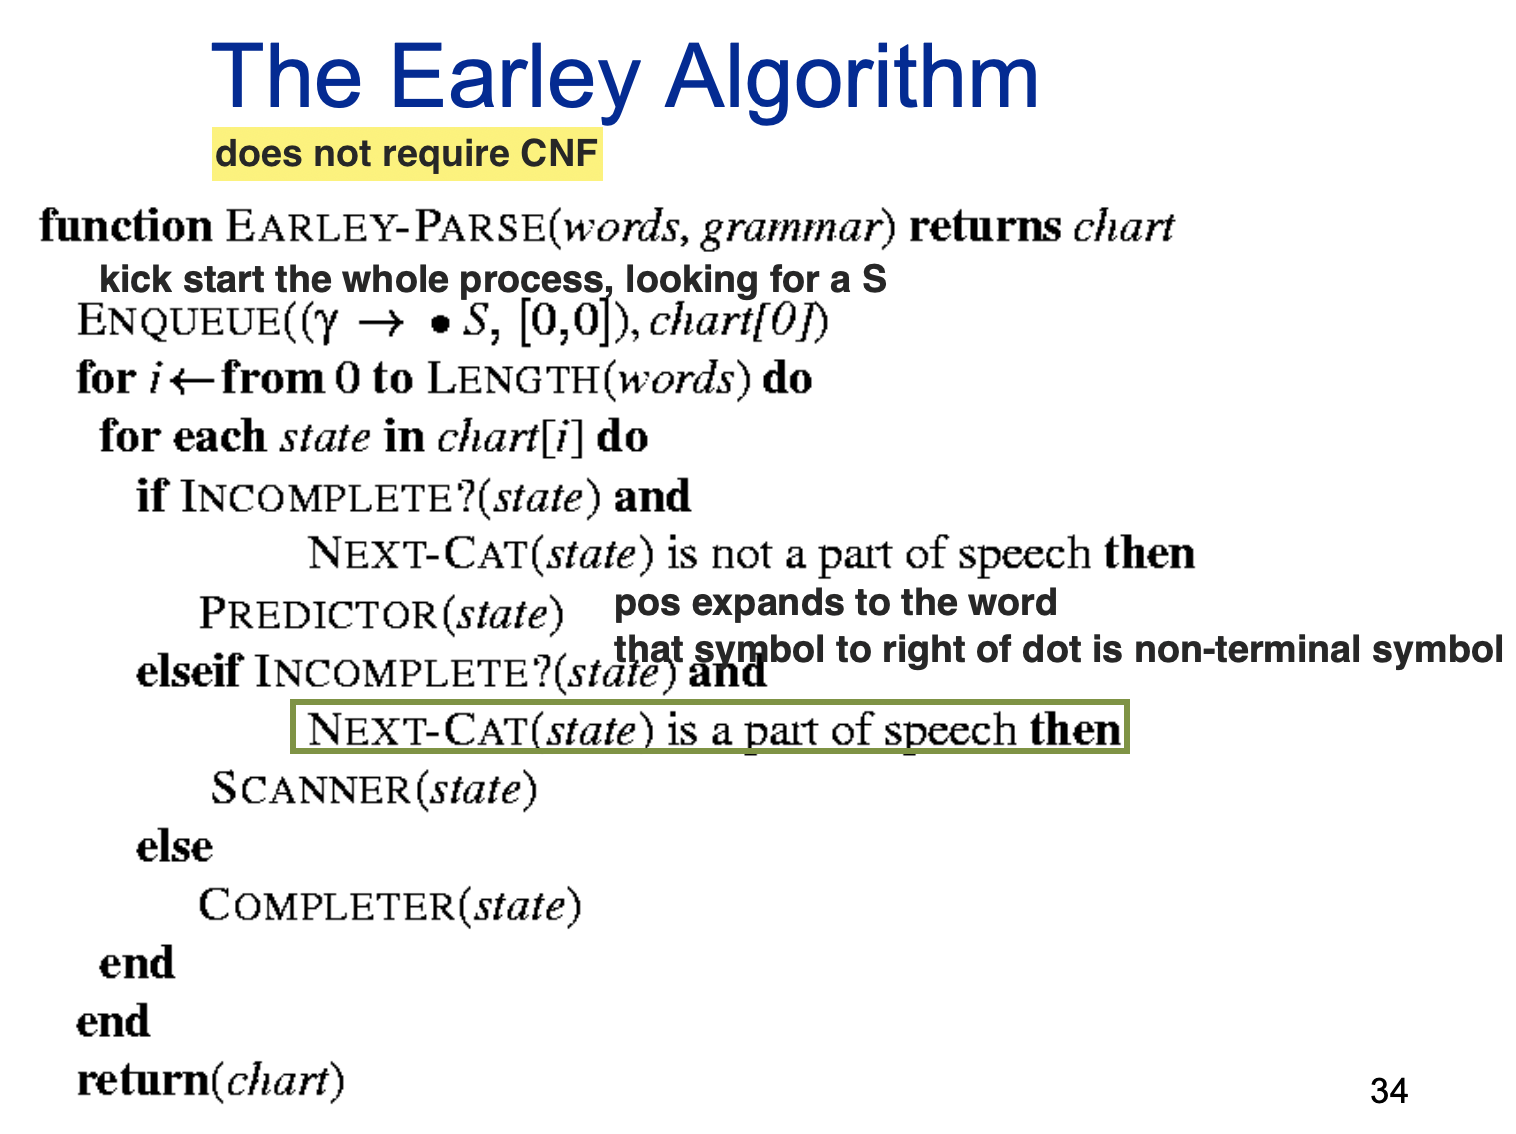
\includegraphics[height=5.5cm]{images/w1_1}
\\
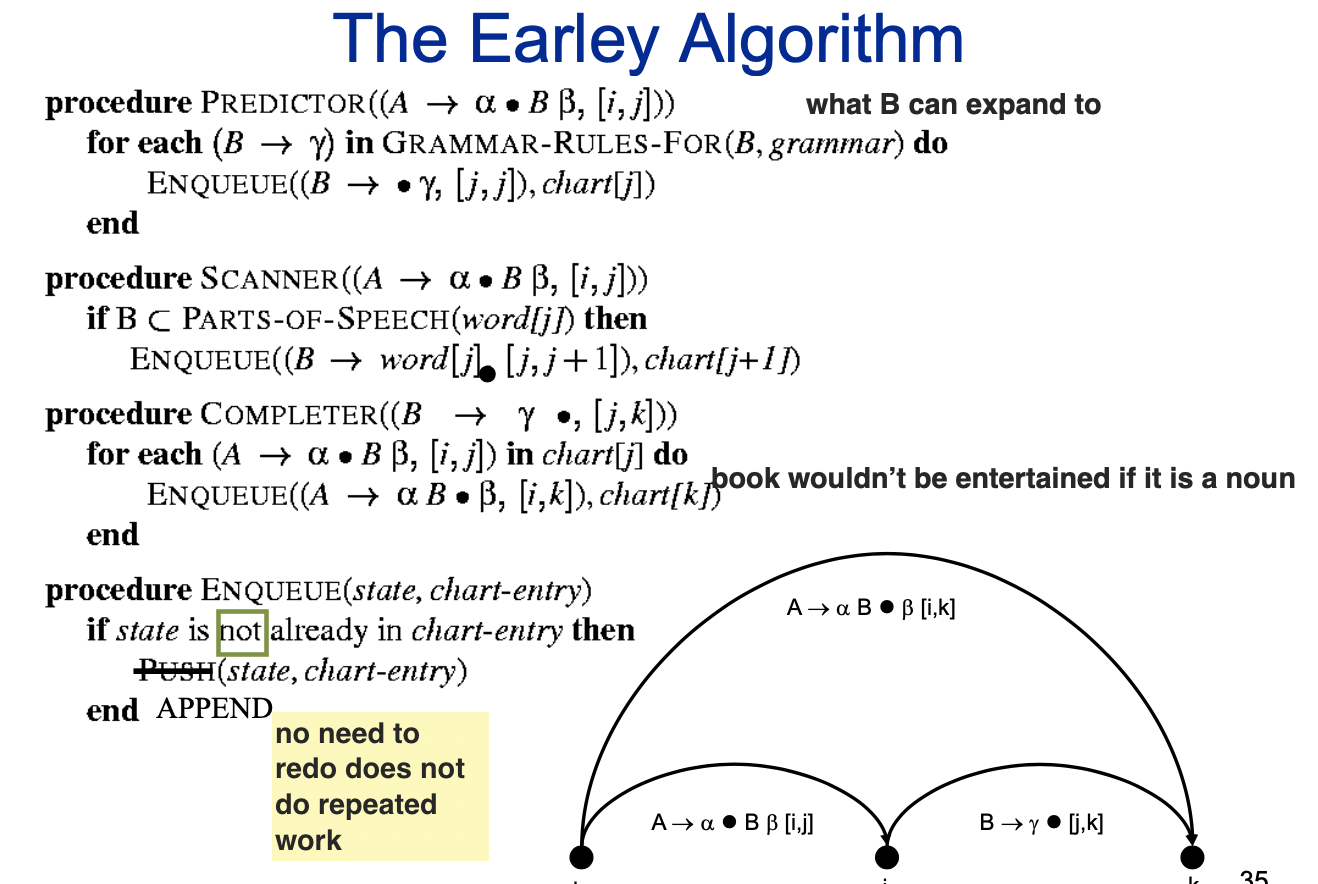
\includegraphics[height=4.5cm]{images/w2}\\
Grammar rules, non-terminal symbol\\
NP - Noun phrase\\
VP - Verb phrase\\
\\
Either have 2 non-terminal symbols or 1 terminal symbol (words)
\subsection*{Garden path sentences}
Reduced relative clause (which was)\\
The horse raced past the barn fell\\
raced used in the passive voice
\subsection*{Decision tree}\\
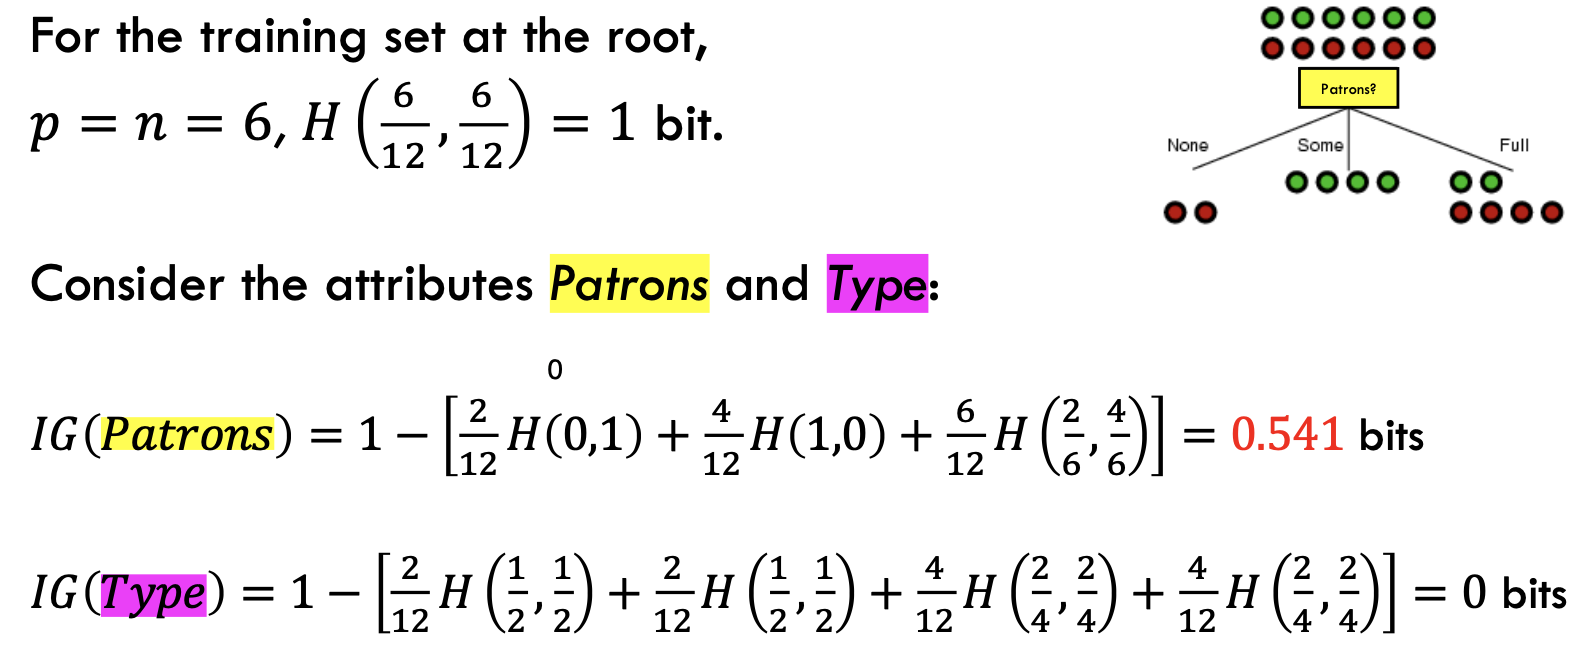
\includegraphics[height=2.5cm]{images/w7}
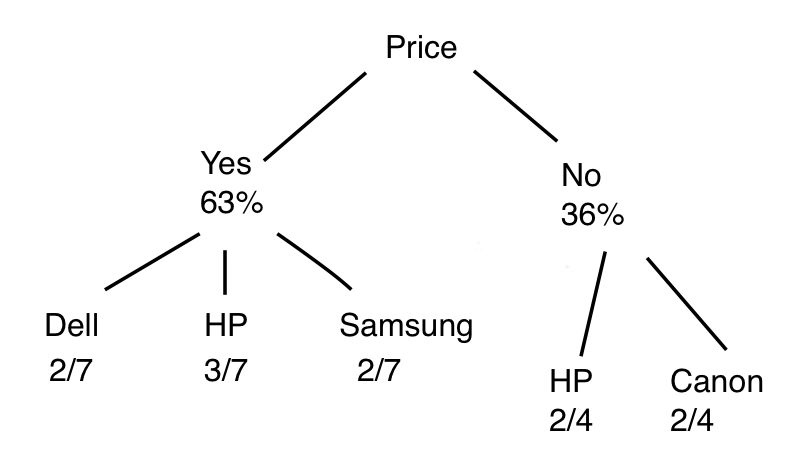
\includegraphics[height=1.5cm]{images/w8}
\subsection*{Every regular language is context free}
Union: $R = R_{1} + R_{2}$\\
$S \rightarrow S_{1} | S_{2}$
\\
Then $S \rightarrow S_{1}$ and $S \rightarrow S_{2}$
\\\\
Concat: R = R_{1}R_{2}\\
$S \rightarrow S_{1}S_{2}$
\\\\
Kleene star:\\
$S \rightarrow S_{1}S_{1} | \epsilon$
\subsection*{Perplexity}
$P(w_{1},...,w_{n})^{-\frac{1}{n}}$ \\
If P(hello) = 1/4, P(there) = 1/4 and there are 30000 names with probability 1/20\\
Then $P(\frac{1}{4} + \frac{1}{4} + \frac{1}{20})^{-\frac{1}{3}$
\subsection*{Semantic Representation}
If CFG, then what is RHS becomes the LHS of the semantic representation\\
1. Determine the POS tags of each word\\
2. Propagate up if there is only 1 RHS\\
3. Apply rules in order, remove first lambda and apply wherever f appears
E.g.\\
NP.sem(VP.sem) then $\lambda$ f $\cdot$ f(Fransca) ($\lambda$ x $\exists$ e Closed(e) ...)
\\
($\lambda$ x $\exists$ e Closed(e) ...) (Frasca)
\\
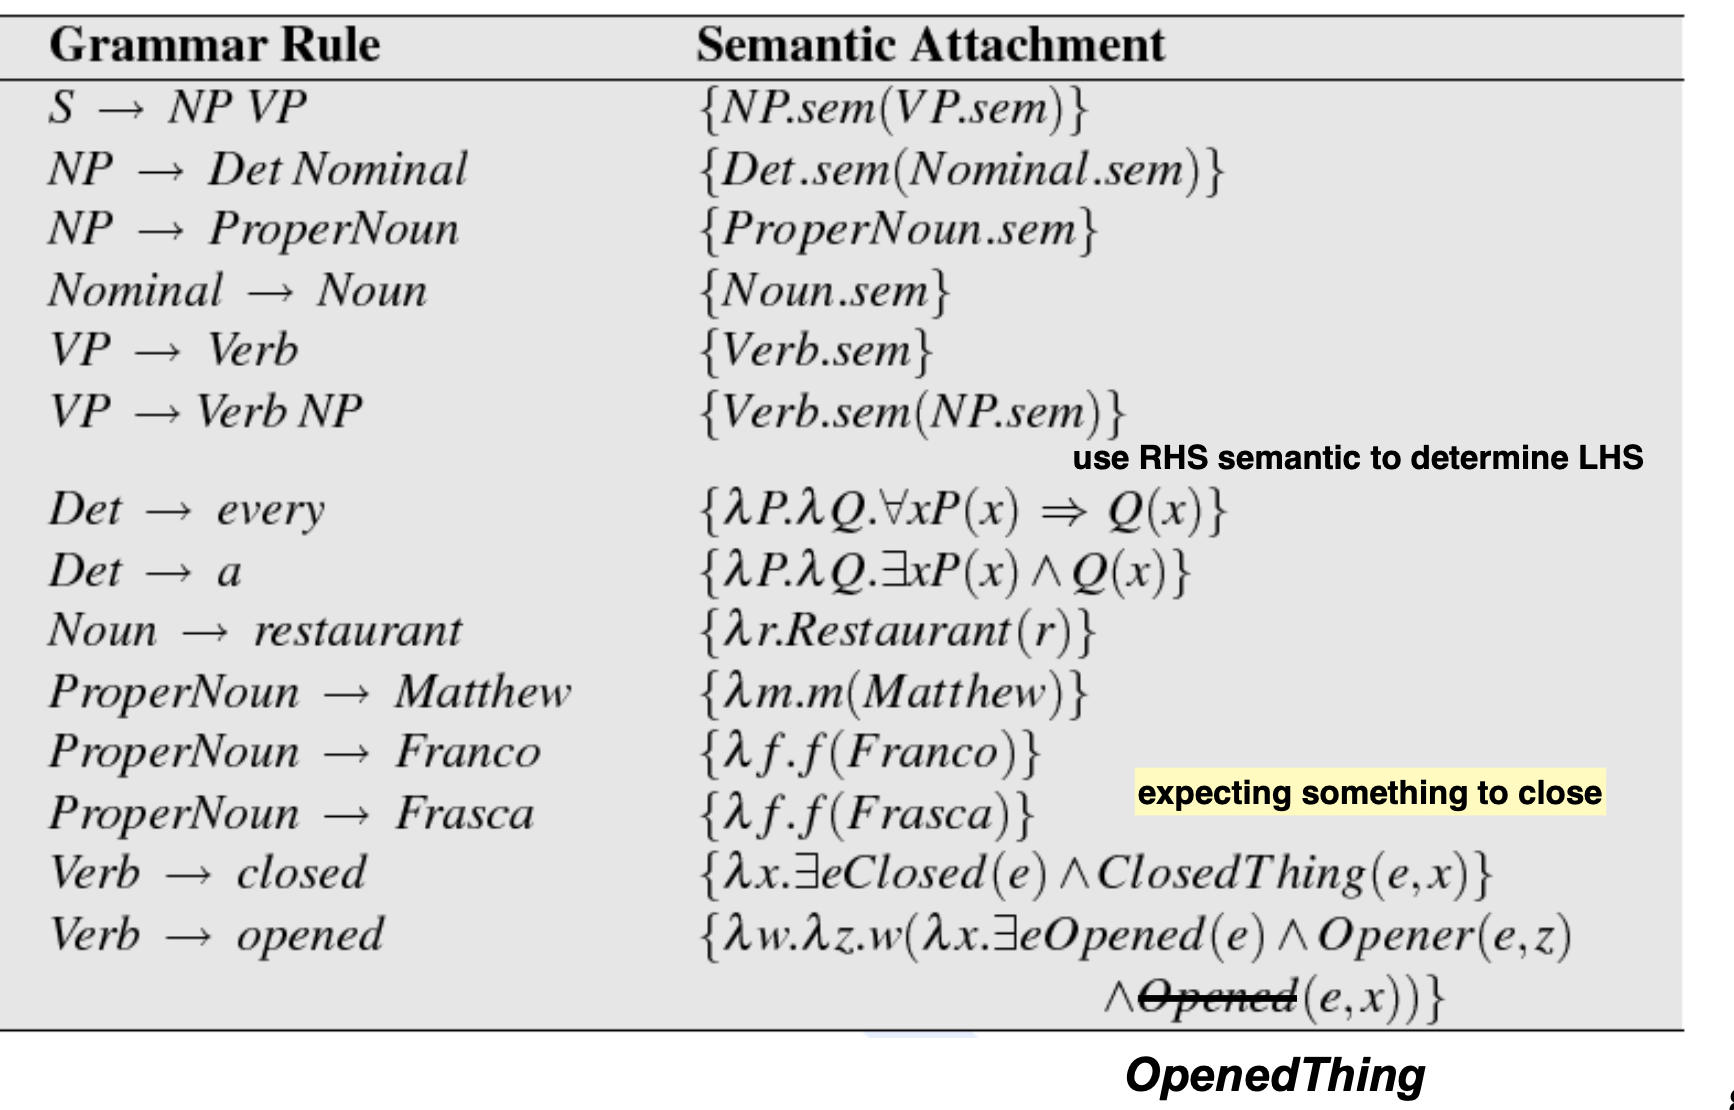
\includegraphics[height=3cm]{images/w14}\\
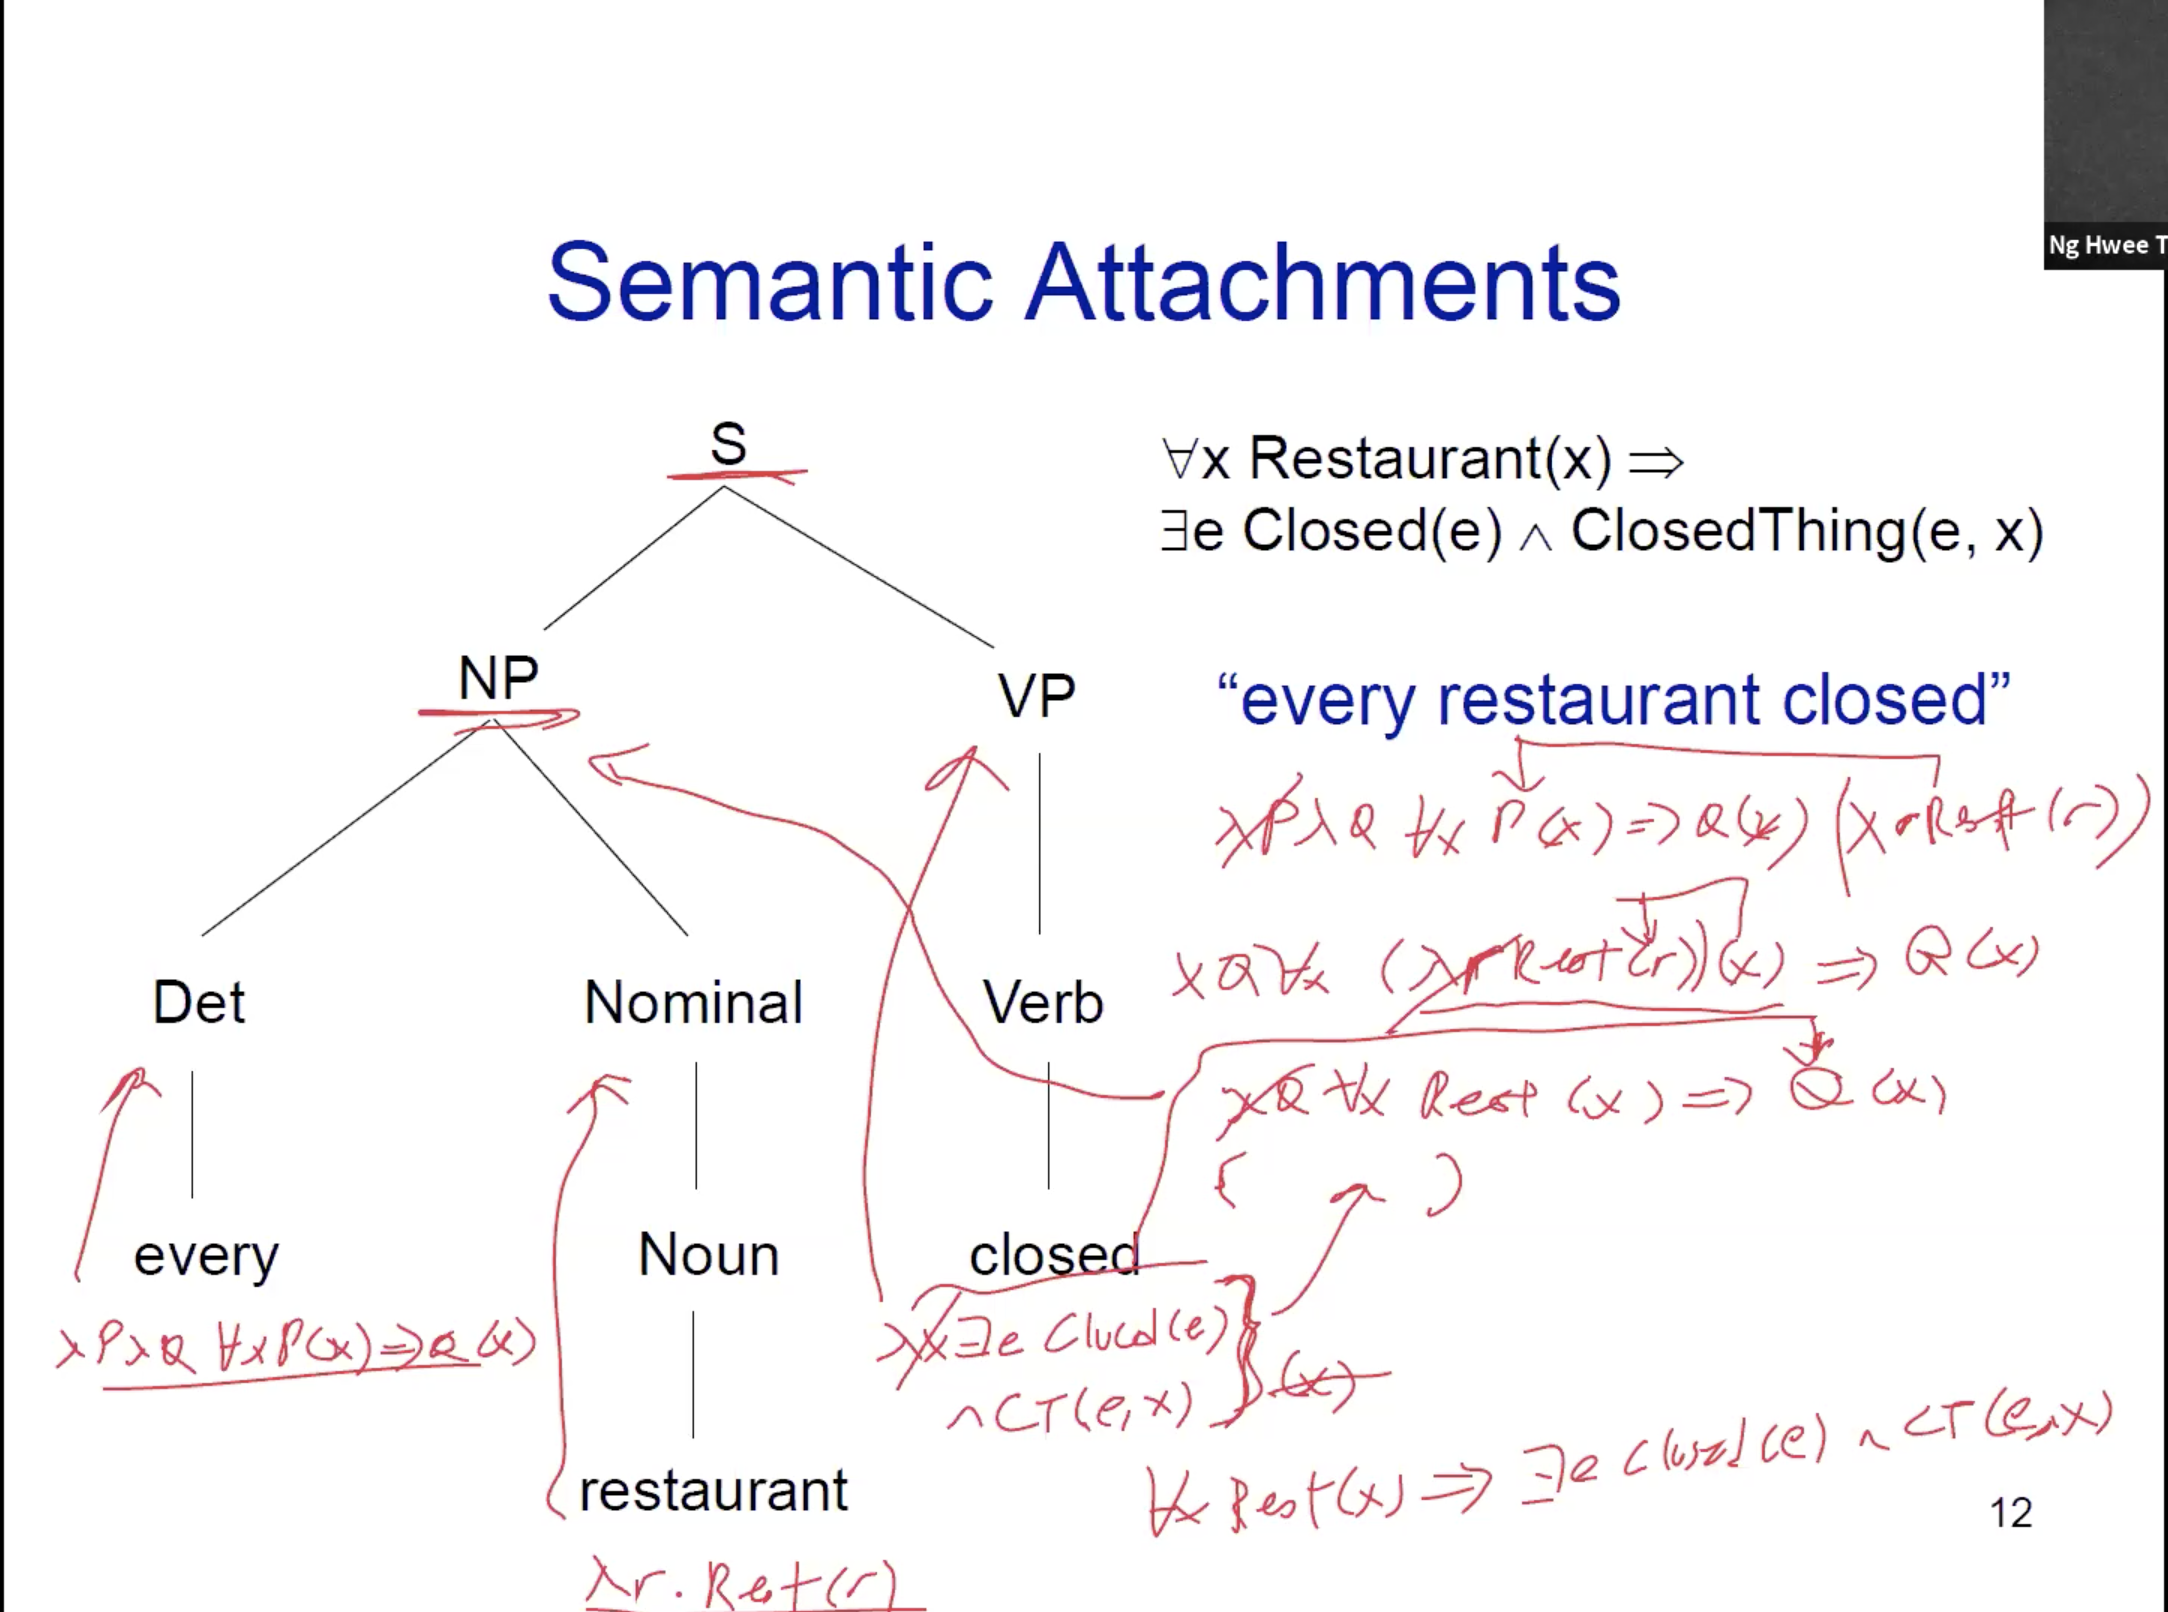
\includegraphics[height=4cm]{images/w12}\\
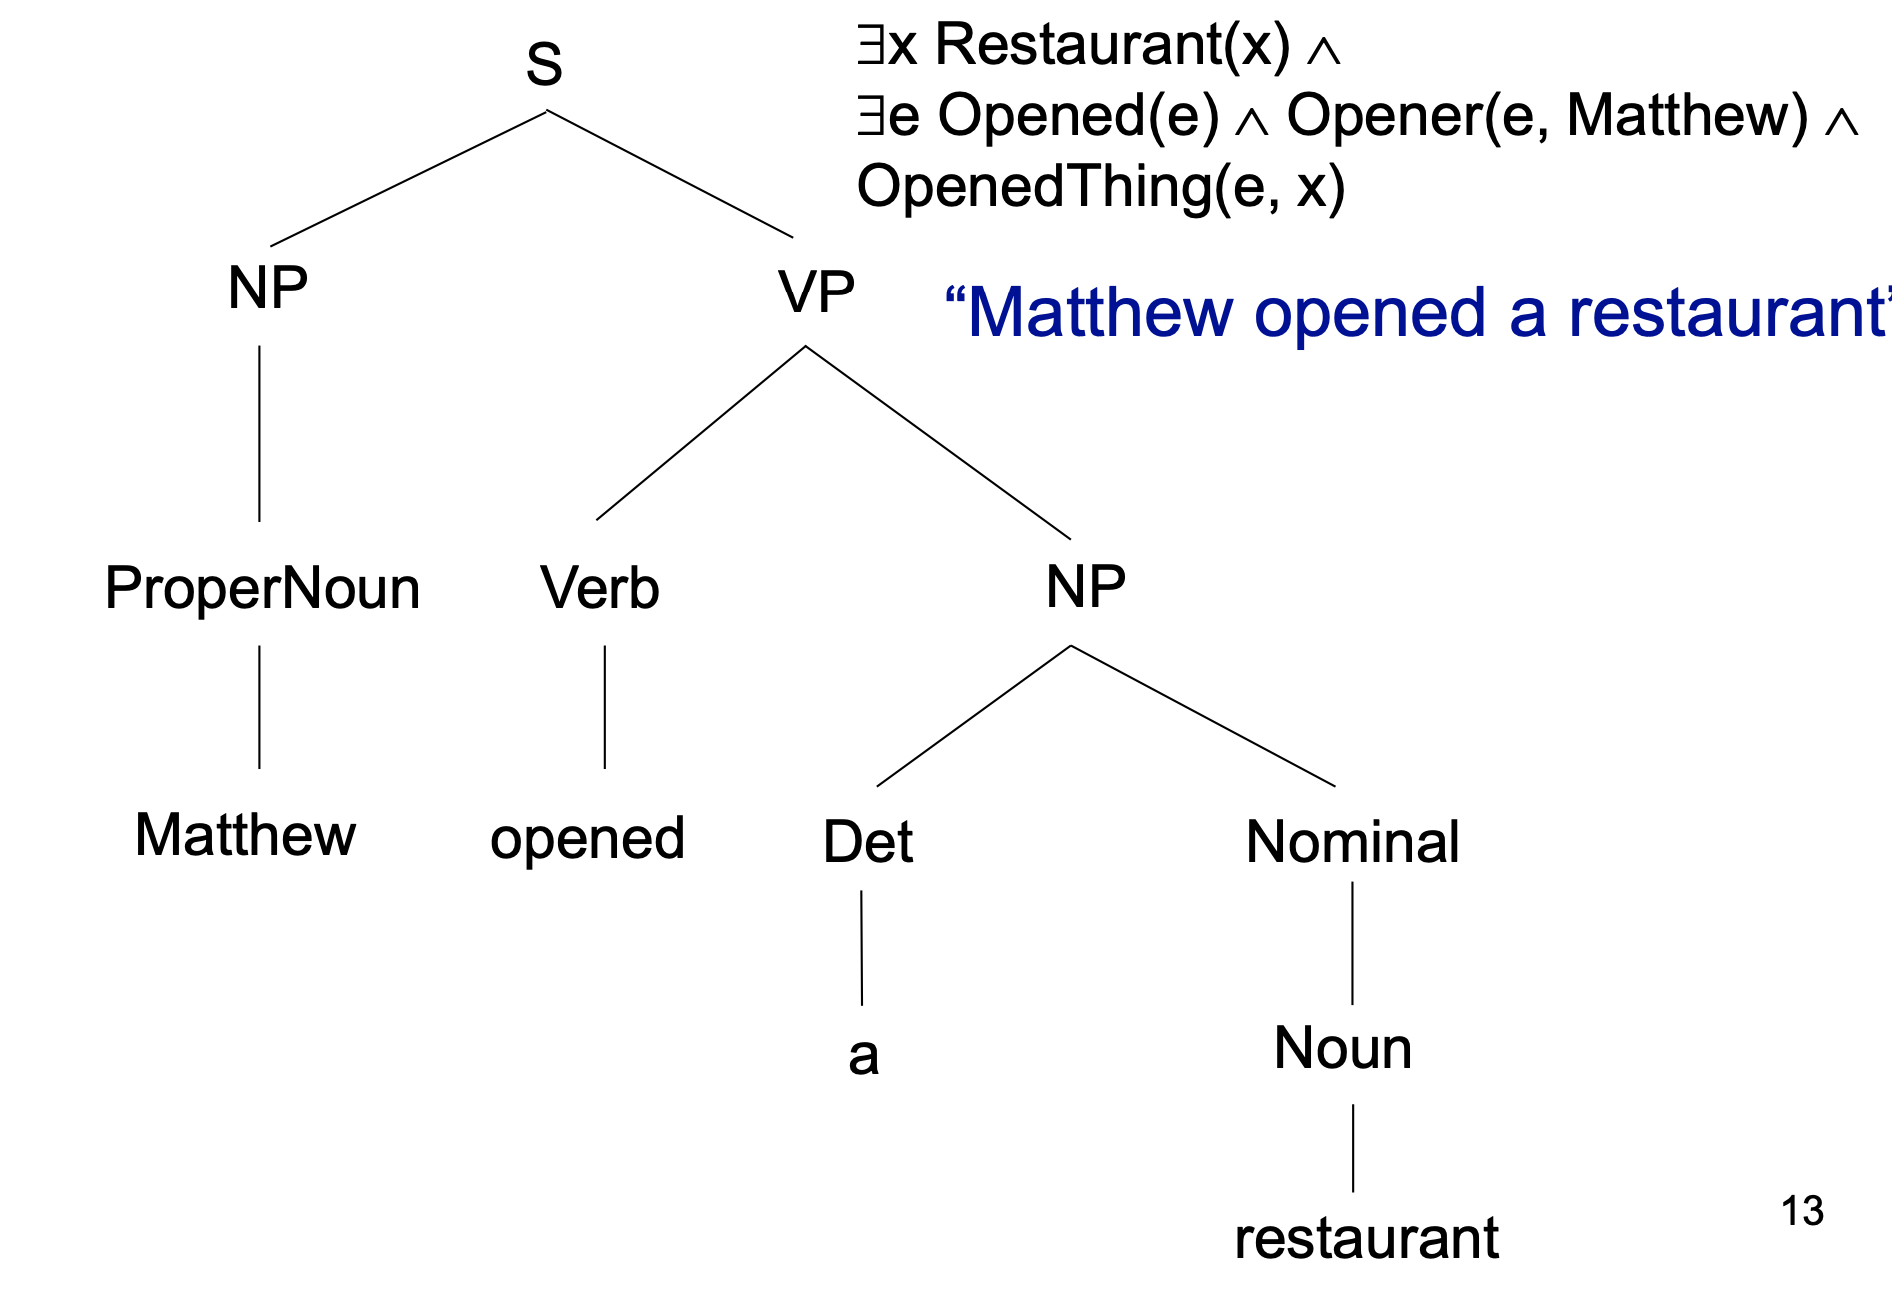
\includegraphics[height=3cm]{images/w15}\\
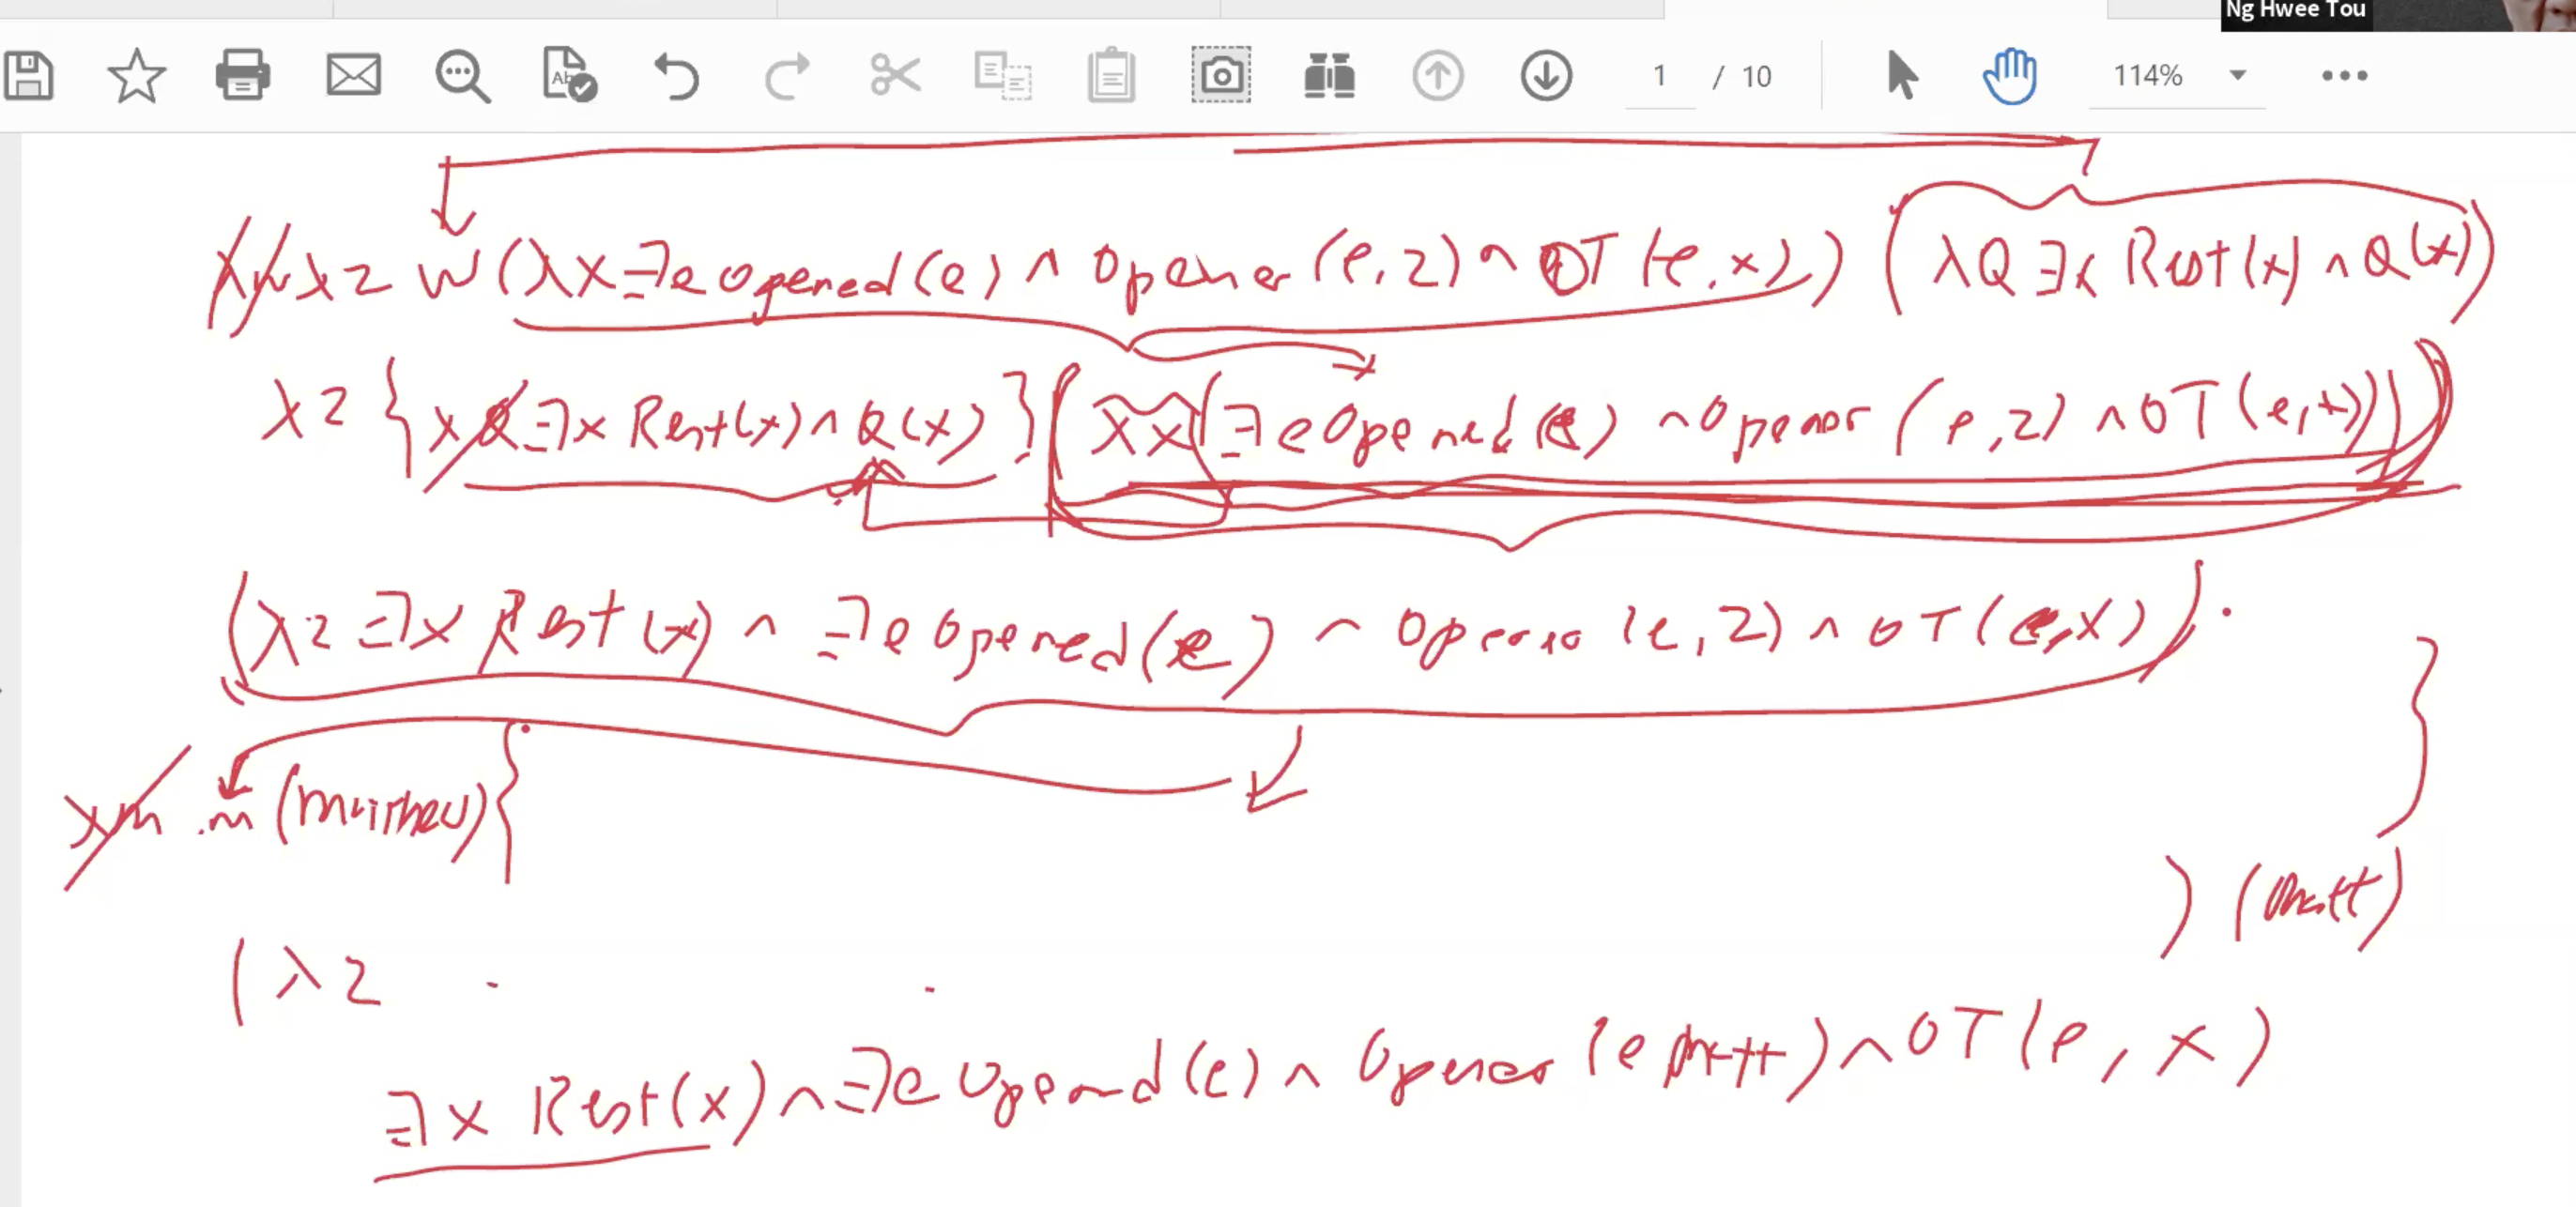
\includegraphics[height=3cm]{images/w13}\\
\subsection*{Constituents Parse trees}
Head word are propagated up the parse tree (RHS to LHS)\\
$NP \rightarrow DT \underline{NN}$
RHS will always be non-terminal symbol unless there is POS tag on LHS\\
E.g. S $\rightarrow$ NP VP
\\
Sometimes there are no direct objects after the verb\\
"he disappeared" instead of "he disappeared mary"\\
Verb decides what types of non-constituents
\subsection*{Head finding}
1. Find the POS tag that expands to each word\\
2. For each grammar rule, add the head child with LHS to be the head\\
3. Add the head word in () beside the new head
\subsection*{Typed Dependency Parse}
Parent is modified by the child\\
!Note! Do not forgot the edge has an arrow pointing from parent to child\\
Who hid? \\
The nominal subj is they and direct obj is letter
\\
on the shelf are more auxiliary things
\\
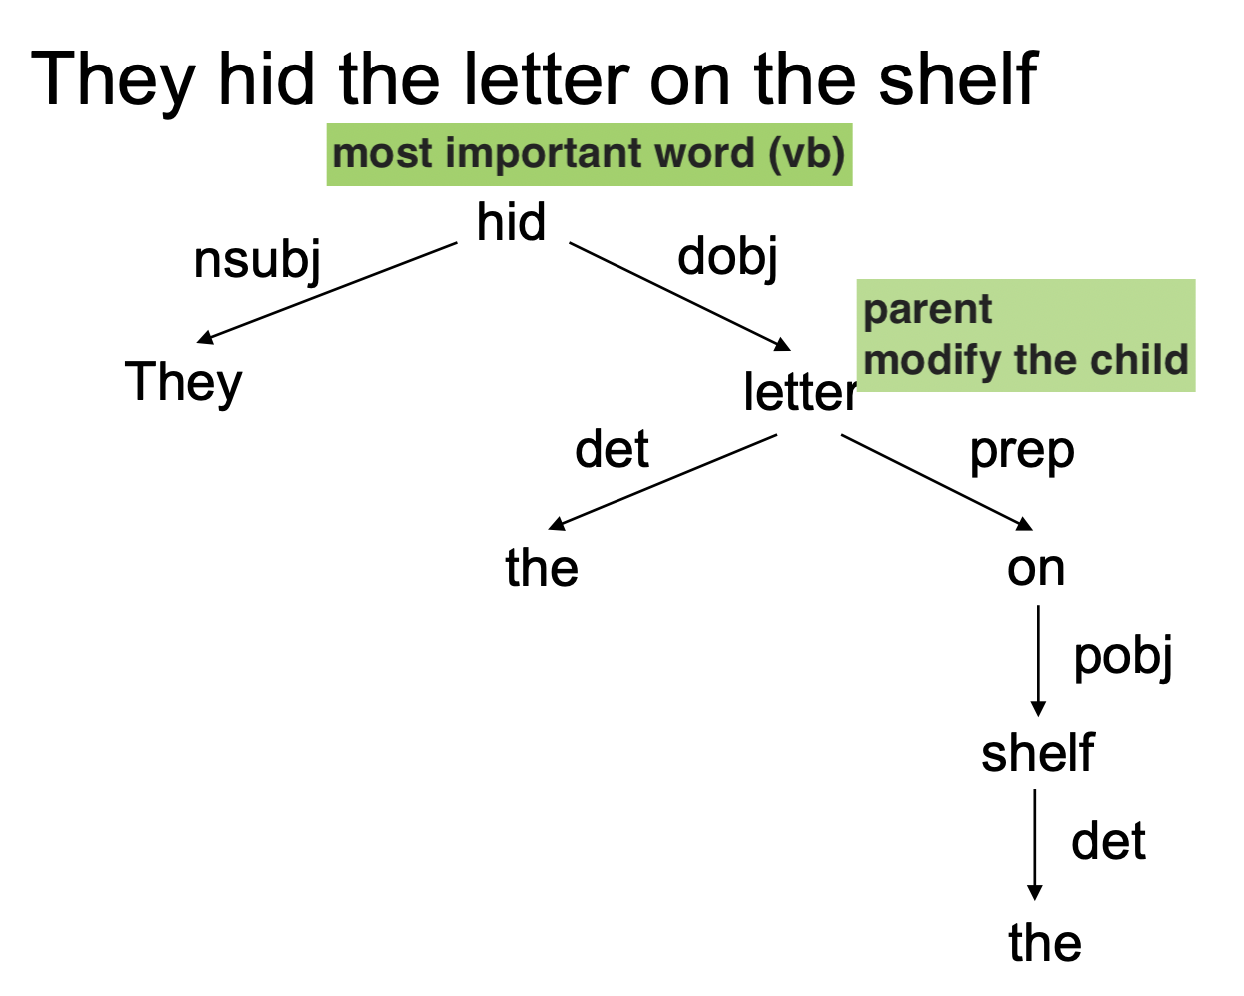
\includegraphics[height=3cm]{images/w10}
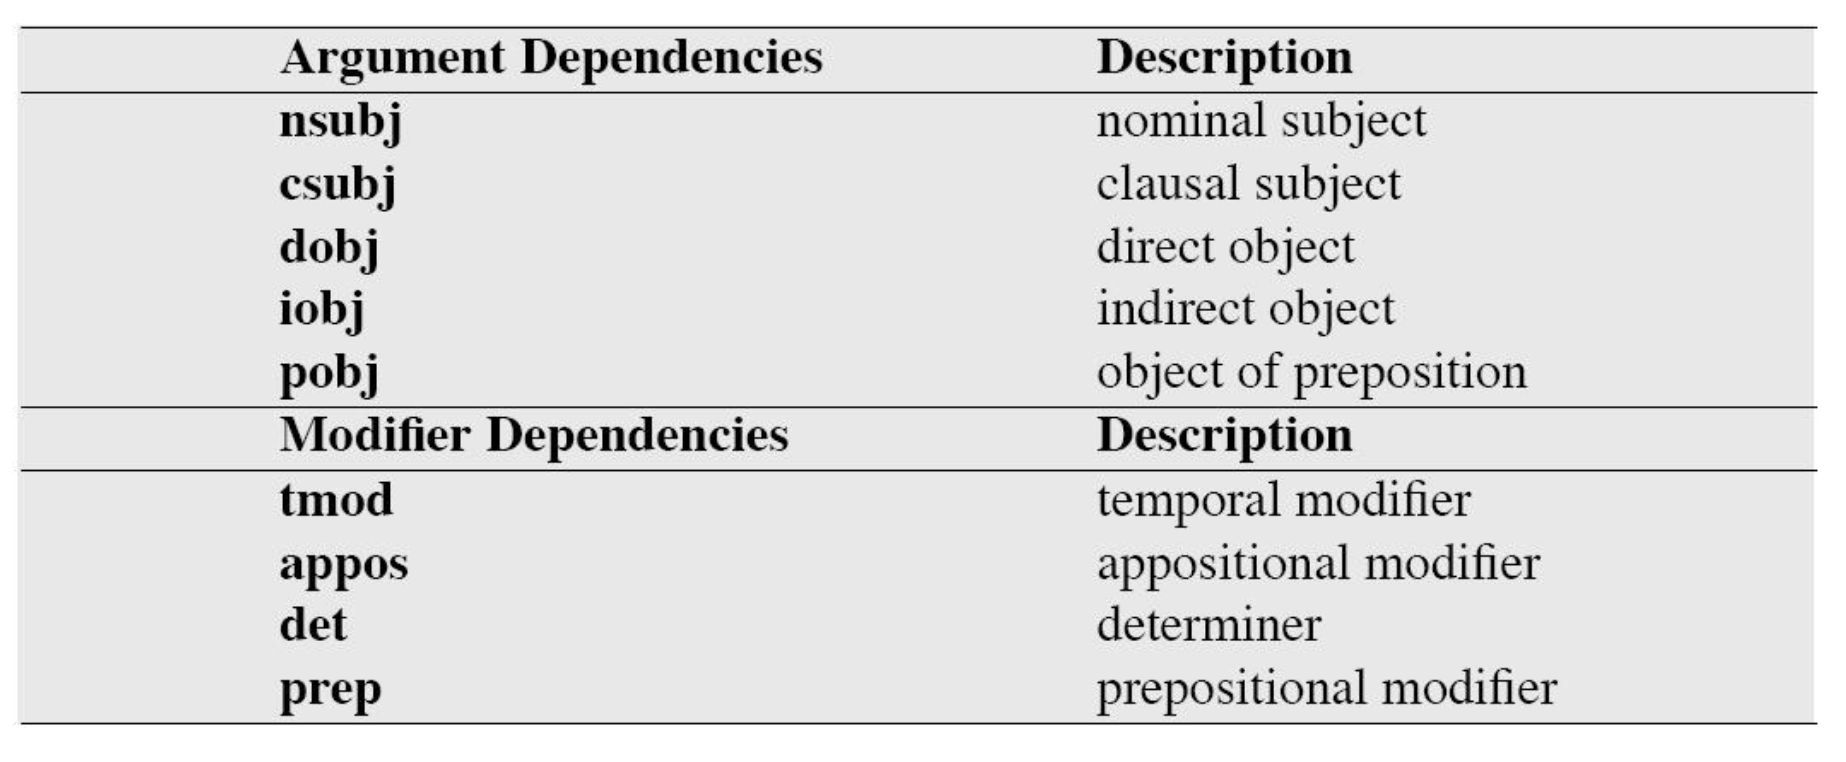
\includegraphics[height=3cm]{images/w9}
\subsection*{Untyped Dependency Parse}
1. Find all the head words\\
2. For every RHS, determine the most important head word then add the other symbols as the children\\
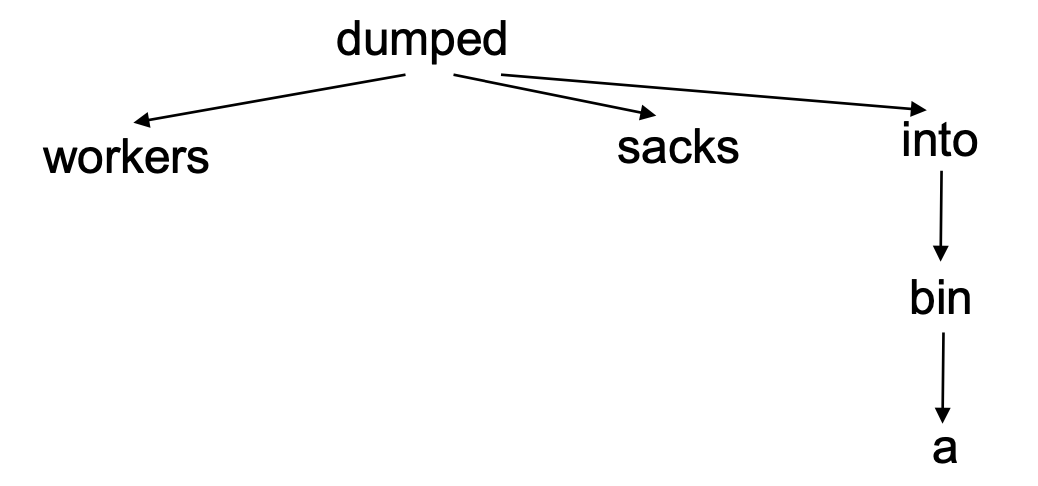
\includegraphics[height=2cm]{images/w11}
\end{multicols*}
\end{document}
